\documentclass[8pt]{amsart}

\usepackage{geometry}
\usepackage{graphicx}
\graphicspath{{./images/}}
\geometry{letterpaper}

\title{Generalized Expressions as an Extension of RegEx, and
    the Use of Token Expressions in Formal Language Translation}
\author{Jordan E Dehmel}

\begin{document}
\maketitle

\section{Abstract}

    The usefullness of RegEx suggests a more generalized class
    of automata and corresponding pattern-matching languages
    where arbitrary objects can be used in place of characters.
    Another instance of this superclass is the machine/language
    pair Token Expression Machine and Token Expressions. These
    operate on tokens (discrete phonemes as parsed by a lexer,
    parser, or tokenizer). This paper outlines the construction,
    control and application of such machines.

    These machines can also be seen as an extension of formal
    language description notations like EBNF. The extension upon
    these forms, of course, is that the machines described
    herein can perform advanced augmentations upon their input
    token streams.

\section{Acronyms}

    Push-Down Automata (PDA), Deterministic Finite Automata
    (DFA), Nondeterministic Finite Automata (NFA), Regular
    Expressions (RegEx), Extended Backus-Naur Form (EBNF).

\section{Abstracting Regular Expressions}

    Regular Expressions (RegEx) are powerful tools for analysis,
    but deeply restricted. A superclass of RegEx, using similar
    notation, could be constructed to be more powerful. This
    superclass, here called Generalize Pattern Matching Automata
    (GPMA), represents a directed cyclic graph wherein each node
    contains either a control instruction or an arbitrary item.
    The only restriction upon this arbitrary item is that it
    must be comparable to any arbitrary item in the input
    stream. Given this quality, an input stream of arbitrary
    (and possibly mixed) datatype can be matched against a
    similarly designed pattern.

    A GPMA could be seen as a typeless generalization of the
    concept of a regular language. We will define a
    GPMA-language (that is to say, a language distinguishable by
    a GPMA) via the following statement: A GPMA-language is a
    set of ordered objects wherein it can be determined whether
    or not any two of the objects are equivalent. No further
    grammatical rules can be applied in the general case.

\section{Token Expressions and TokEx Machines}

    Using the above definition of GenEx, we can easily recognize
    regular expressions as instances of a larger superclass. A
    related family within this superclass are the TokEx (Token
    Expressions). We shall detail these here.

    A compiled Tokex machine is a directed graph, with the
    "left" node being the beginning and the "right" node being
    the end. The current node (or state) of the machine moves
    from left to right based on the input. Most nodes in the
    graph are literals (which can only be moved to if the input
    token matches), but there are also wildcard nodes,
    special-case nodes (for instance the beginning and end) and
    variable/memory control nodes. The variable/memory control
    nodes interface with the bank of linked lists within the
    machine. They allow the input memory to be cleared and for
    the full input memory list to be pushed onto the end of a
    variable stack. The input of a Tokex machine is a token
    stream.

    Due to the memory and variable system, a Tokex machine is
    technically a PDA. However, its design philosophy is most
    akin to DFA/NFA due to its applications.

\section{Applications}

    The fact that a Tokex Machine operates only on token streams
    is both an advantage and a disadvantage. One one hand, it
    means that it is more efficient and powerful than RegEx
    in situations where the input text has already been
    tokenized, but it also may incur additional overhead when
    compared to RegEx in situations where the input text has not
    yet been tokenized. We will largely be focusing on the
    former case here.

\section{Suggested Notation}

    Like a DFA without RegEx, the Tokex machine is near-useless
    without a control language. This paper proposes the
    following set of notations. A simple algorithm can be
    constructed to compile a Tokex machine from this notation in
    quasi-linear time. The below notation is optimized to be
    parsed by the same tokenizer as the Tokex's input token
    stream (hence the use of the uncommon delinator $\$$).

    \subsection{Whitespace}

    All whitespace is to be erased by the TokEx parser, and thus
    the language needs additional symbols to represent it. This
    paper suggests \verb|\s| for spaces, \verb|\t| for tabs, and
    \verb|\n| for newlines.

    \subsection{Input Pattern Notation}

    The below table displays TokEx input pattern notation, which
    is used to describe a single input patter.

\begin{center}
\begin{tabular}{|l|l|l|}
    \hline
    Notational Token    & Name          & Meaning \\
    \hline
    $\verb|$.|$
        & Wildcard
        & Matches any one token \\

    $\verb|$*|$
        & Start glob
        & Repeat the previous expression zero or more times \\

    $\verb|$+|$
        & Plus glob
        & Repeat the previous expression one or more times \\

    $\verb|$?|$
        & Optional glob
        & Repeat the previous expression zero or one times \\

    $\verb|$( ... $)|$
        & Subexpression
        & Treat this block as a single expression \\

    $\verb|$a()|$
        & Composition
        & Creates another machine of the given pattern, which
          must match in order for this pattern to. This may be
          recursive \\

    $\verb:$( ... $| ... $):$
        & Subexpressions
        & Use one of multiple subexpressions \\

    $\verb|$[ ... $]|$
        & Suit
        & Match any of the items within \\

    $\verb|$[^ ... $]|$
        & Negated suit
        & Match anything but the items within \\

    $\verb|${ a $, b $}|$
        & Repetition
        & Match any number of repetitions $n$
          where $a \leq n \leq b$ \\

    $\verb|$~|$
        & Clear memory
        & Clears the list of previously matched tokens \\

    $\verb|$>name|$
        & Pipe memory
        & Appends the list of previously matched tokens to a
          variable \\ 

    $\verb|$-'TAG'>A|$
        & Add tag
        & Adds the contents of the variable $A$ to the tag set
          $TAG$ \\

    $\verb|$?-'TAG'>A|$
        & Check for tag
        & If $A$ is not in the tag set $TAG$, this is not a
          match \\

    $\verb|$?^-'TAG'>A|$
        & Negated check for tag
        & If $A$ is in the tag set $TAG$, this is not a match \\

    $\verb|$A-'ATN'>B|$
        & Add association
        & Adds a link from $A$ to $B$ in association set
          $ATN$ \\

    $\verb|$?A-'ATN'>B|$
        & Check for association
        & If $A$ does not have an association with $B$ under the
          tag $ATN$, this is not a match \\

    $\verb|$?^A-'ATN'>B|$
        & Negated check for association
        & If $A$ has an association with $B$ under the tag
          $ATN$, this is not a match \\

    $\verb|$A-'ATN'>>B|$
        & Fetch association target
        & Appends the target of $A$ under the association $ATN$
          onto the variable $B$ \\

    \hline
\end{tabular}
\end{center}

    Anything not beginning with the special character \verb|$|
    is to be considered a literal by the TokEx executer.

    \textbf{Note:} The only "card" here which relies on external
    infrastructure is composition. This may result in
    expressions whose validity is indeterminable when taken out
    of context. However, it also greatly improves readability.

    \subsection{Output Pattern Notation}

\begin{center}
\begin{tabular}{|l|l|l|}
    \hline
    Notational Token    & Name          & Meaning \\
    \hline
    $\verb|$name|$
        & Variable
        & Inserts the contents of the variable \verb|name| \\

    $\verb|$<delim|$
        & Concatenation
        & Merges the following token or variable onto the end
          of the previous one, using the provided deliminator or
          no deliminator by default \\

    \hline
\end{tabular}
\end{center}

    Any token which does not begin with the special character
    \verb|$| is considered a literal.

    \subsection{Full TokEx Notation}

    Full TokEx notation takes advantage of both input an output
    rule notation, and allows for more advanced procedures like
    composition. This is what would be loaded as a file by a
    TokEx executer. This is a file format which expects all
    input and output rules to be enclosed in single quotes, or
    triple-single-quotes for multi-line rules. It uses
    semicolons to signify the end of a given rule. The following
    example gives a comprehensive look at the file format.

\begin{verbatim}
$rule_name() := ' input pattern ' -> ' output pattern ';

$rule_name() :=
    '''
    input pattern
    which takes
    several lines
    '''
    ->
    '''
    output pattern
    which takes
    several lines
    ''';

// Comment
% Also a comment

$rule_which_has_no_output() :=
    '''
    Hello , world !
    ''';

// Note: Regex rules cannot have output.
// They operate on only one token, and cannot be multi-line.
$regex_only_rule() := r'some regex here';

\end{verbatim}

    This paper suggests the file extension \verb|.te| for such
    files. When writing some rule $R$ in a mathematical context,
    this paper suggests the notation
    $R : \verb|"input"| \to \verb|"output"|$.

\section{The Double Counting Problem}

    Consider the patterns $P_1 : \verb|"A B C"| \to \verb|"1"|$
    and $P_2 : \verb|"B C D"| \to \verb|"2"|$ on the text
    \verb|"A B C D"|. The first three tokens would result in
    $P_1$ being matched, while the second through fourth tokens
    would result in $P_2$ being matched. Since either of these
    rules would cause the replacement of their match and
    invalidate the other, it is necessary that we have a
    deterministic way of determining which would prevail. This
    is the "double counting problem" when running multiple
    TokEx machines simultaneously. For the purposes of this
    paper, we will resolve this issue by resetting the states of
    all machines when a modifying machine reaches a match state.
    Thus, there will be no overlapping matches. We will not
    reset the state when a non-modifying pattern matches.
    Additionally consider the patterns
    $P_3 : \verb|"A B C"| \to \verb|"3"|$ and
    $P_4 : \verb|"A B C D"| \to \verb|"4"|$ on the text
    \verb|"A B C D"|. Even though they began matching at the
    same location, $P_1$ would match and augment the input token
    stream before $P_2$ could. Due to our previously described
    rule, however, $P_2$ would be fully reset before it could
    conclude. Finally, consider the patterns
    $P_5 : \verb|"A B C"| \to \verb|"5"|$ and
    $P_6 : \verb|"A B C"| \to \verb|"6"|$ on the text
    \verb|"A B C"|. Both $P_5$ and $P_6$ would conclude at the
    same token, and would suggest different augmentations. This
    is to be considered an invalid description, and thus these
    two rules cannot exist in a valid TokEx system together.

    A valid TokEx system is defined as a set of TokEx rules
    wherein no rules can cause ambiguous output and an "entry"
    rule is defined. This means that the output of a valid TokEx
    system is a deterministic function of its rules and input
    token stream. The entry point rule is necessary in order to
    know which rule is to be searched for. For the purposes of
    this paper, we will denote such a rule as \verb|$MAIN()|.

\section{Examples}

    \subsection{JSON}

    This examples comes from the EBNF representation of JSON.
    This demonstrates that TokEx patterns are at least as
    powerful as EBNF.

\begin{verbatim}
$MAIN() := ' $object() $* ';

$value() :=
    '''
    $(
        $string() $|
        $number() $|
        $object() $|
        $array() $|
        true $|
        false $|
        null
    $)
    $whitespace()
    ''';

$whitespace() := ' $( \w $| \t $| \n $) $* ';

$string() := r'"(\\"|.)*"';

$number() := r'-?([0-9]*\.[0-9]*|[1-9][0-9]*)([eE][+-][1-9][0-9]*)?';

$object() :=
    '''
    {
        $(
            $( $object_item() , $whitespace() $) $*
            $object_item()
        $) $?
        $whitespace() $*
    }
    ''';

$object_item() := ' $string() : $value ';

$array() :=
    '''
    [
        $(
            $( $value() , $) $*
            $value()
        $) $?
    ]
    ''';

\end{verbatim}

    Although this TokEx system is non-transformative (does not
    contain any transformative rules), it still demonstrates the
    power of TokEx.

    \subsection{Bootstrapping}

    The following TokEx system matches syntactically valid TokEx
    systems, given that the lexer being used recognizes triple
    quoted string literals.

\begin{verbatim}
$MAIN() :=
    '''
    $tokex_system() $* $main_statement() $tokex_system() $*
    ''';

// A tokex system is a series of statements.
$tokex_system() := ' $( $statement() \n $) $* ';

// A statements is an ID followed by a definition, either TokEx
// or RegEx.
$statement() :=
statement =
    '''
    $id() := $( $tokex_body() $| $regex_str_lit() $) ;
    ''';

$main_statement() :=
    '''
    \$main() := $tokex_body();
    ''';

// An ID is a dollar sign followed by characters followed by
// parenthesis.
$id() := r'\$[a-zA-Z0-9_]\(\)';

// A TokEx body is an input rule optionally followed by an
// output rule.
$tokex_body() := ' $rule() $( -> $rule() $) $? ';

// A rule is either a single quoted string literal or a triple
// quoted string literal.
$rule() :=
    '''
    $( $single_str_lit() $| $triple_str_lit() $)
    ''';

// A single-quoted string literal.
$single_str_lit() := r'\'.*\'';

// A triple-quoted string literal.
$triple_str_lit() := r'\'\'\'.*\'\'\'';

// A RegEx literal.
$regex_str_lit() := r'r\'.*\'';

\end{verbatim}

    This system is also non-transformative.

    \subsection{De-Parenthesize}

    The following TokEx system removes all redundant
    parenthesis.

\begin{verbatim}
$entry() := ' ( $recursive() ) ';

$recursive() := '( $~ $recursive() $>contents )' -> '$contents';
\end{verbatim}

    This would reduce the input text "(((((foobar)))))" to
    "(foobar)". This is a transformative system, and
    demonstrates that TokEx systems are more powerful than
    RegEx.

    \section{Node Construction}

\begin{figure}[h]
    \caption{Node diagram of a single literal.}
    \centering
    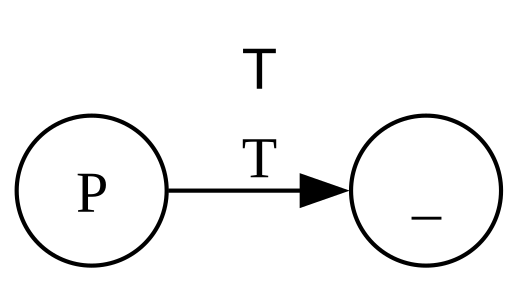
\includegraphics[width=0.35\textwidth]
        {diagrams/base}
    \label{fig:literal_nd}
\end{figure}

\begin{figure}[h]
    \caption{Node diagram of a "plus" glob.}
    \centering
    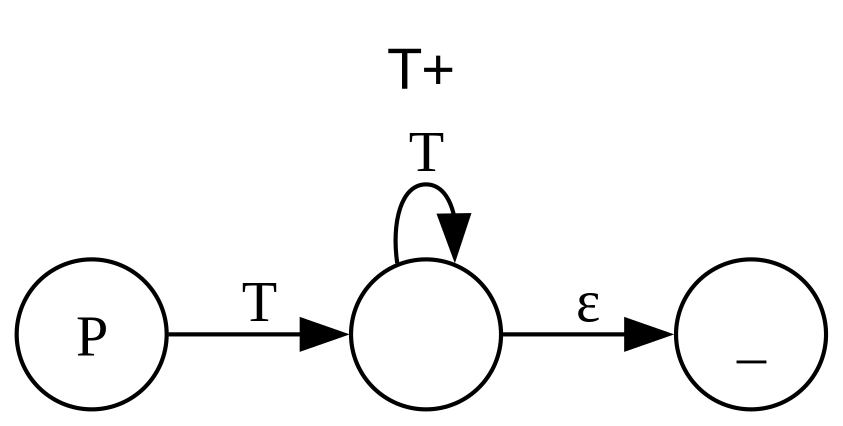
\includegraphics[width=0.35\textwidth]
        {diagrams/plus}
    \label{fig:plus_nd}
\end{figure}

\begin{figure}[h]
    \caption{Node diagram of a "question" glob.}
    \centering
    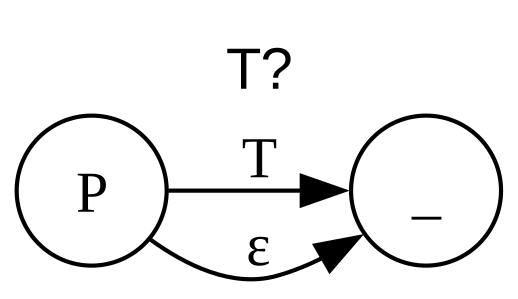
\includegraphics[width=0.35\textwidth]
        {diagrams/question}
    \label{fig:question_nd}
\end{figure}

\begin{figure}[h]
    \caption{Node diagram of a "star" glob.}
    \centering
    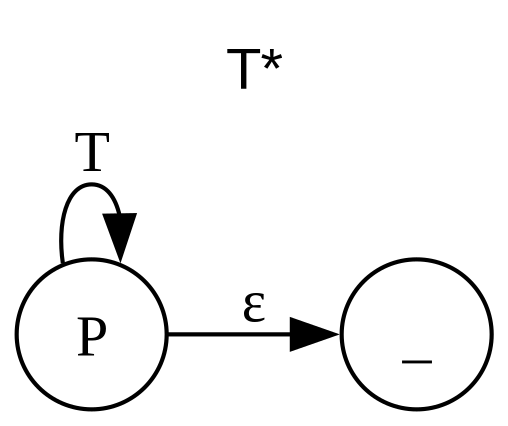
\includegraphics[width=0.35\textwidth]
        {diagrams/star}
    \label{fig:star_nd}
\end{figure}

\begin{figure}[h]
    \caption{Node diagram of a "suit".}
    \centering
    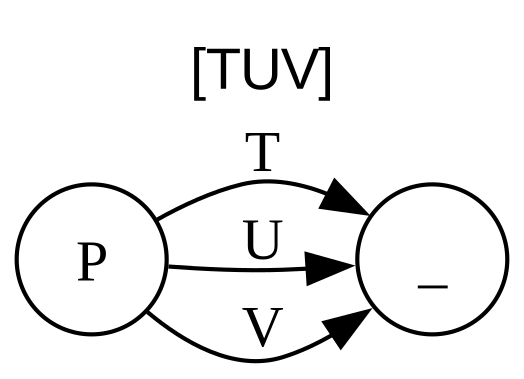
\includegraphics[width=0.35\textwidth]
        {diagrams/suit}
    \label{fig:suit_nd}
\end{figure}

    Let us assume that a given expression can be parsed into
    discrete units which can then be assembled together into one
    DFA. Each unit will have access to one input node, and will
    be responsible for returning one output node. We will only
    worry about forward progression through the graph for now.
    Each unit is allowed to use epsilon transitions (transitions
    which occur without input) in order to maintain the
    invariant. The output node of one graph will be used as the
    input node of the next. Each graph unit will be responsible
    for any transitions out of the input node and for creating
    the output node. These units can be broken down into a few
    base cases, then recursively constructed into a full
    expression.

    (1) Deconstruct expression into subexpressions
    (2) Construct partial node diagrams
    (3) Knit node diagrams
    (4) Perform epsilon closure

\end{document}
